%%% Platform.tex --- 
%% Version: $Id: Platform.tex,v 0.0 2012/05/10 01:10:42 tangboyun Exp$
%% Copyright : (c) 2012 Boyun Tang
%% License : BSD-style
\documentclass{standalone}
\usepackage{tikz}
\usetikzlibrary{mindmap,shadows,shapes.arrows,shapes.geometric,shapes.misc,matrix,arrows,positioning,calc,decorations.pathreplacing,petri}
\usepackage{graphicx}
\usepackage{times}
\usepackage{xcolor}
\begin{document}

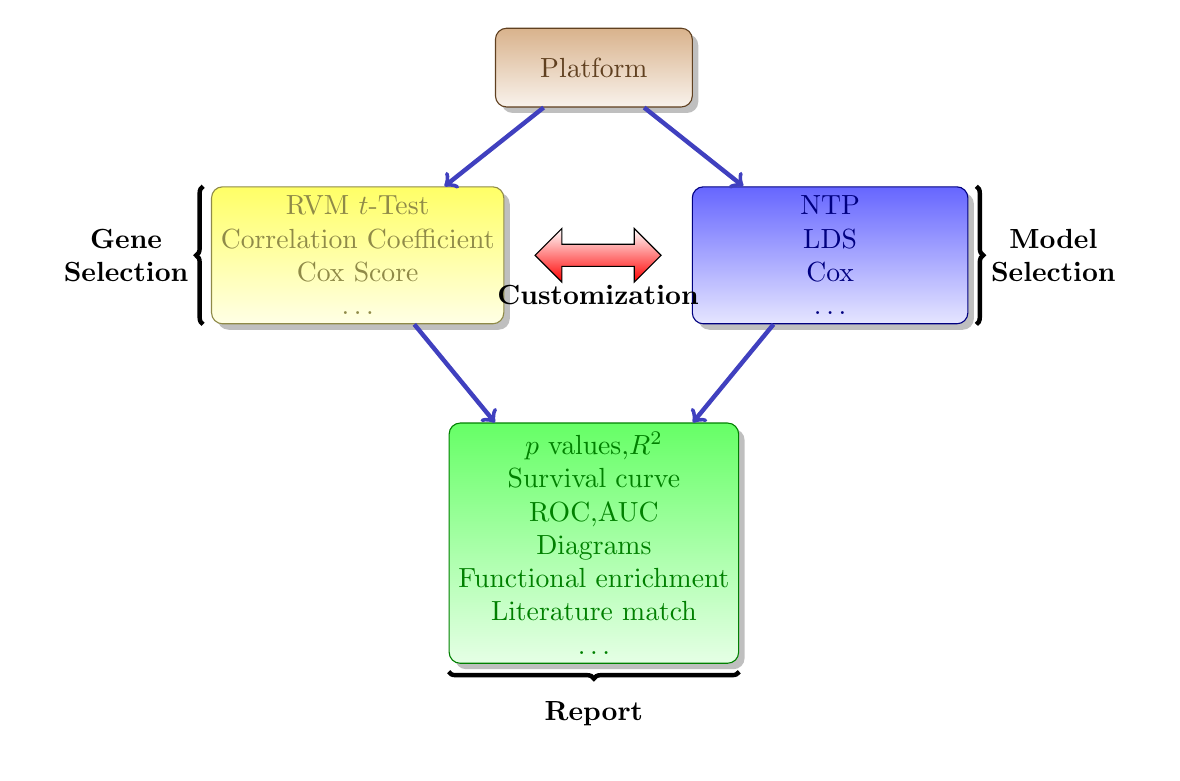
\begin{tikzpicture}[
  every node/.style={minimum width=2.5cm,minimum height=1cm,align=center,},%
  dr/.style={drop shadow},%
  e/.style={->,ultra thick,rounded corners,draw=blue!50!gray},%
  cl/.style={cylinder,aspect=.3,shape border rotate=90,},%
  re/.style={rounded corners,},%
  r/.style={top color= red!60,bottom color= red!10,draw=red!50!black,%
    text=red!50!black,},%
  g/.style={top color= green!60,bottom color= green!10,draw=green!50!black,%
    text=green!50!black,},%
  b/.style={top color= blue!60,bottom color= blue!10,draw=blue!50!black,%
    text=blue!50!black,},%
  br/.style={top color= brown!60,bottom color= brown!10,draw=brown!50!black,%
    text=brown!50!black,},%
  v/.style={top color= violet!60,bottom color= violet!10,draw=violet!50!black,%
    text=violet!50!black,},%
  o/.style={top color= orange!60,bottom color= orange!10,draw=orange!50!black,%
    text=orange!50!black,},%
  ye/.style={top color= yellow!60,bottom color= yellow!10,draw=yellow!50!black,%
    text=yellow!50!black,},%
  p/.style={top color= pink!60,bottom color= pink!10,draw=pink!50!black,%
    text=pink!50!black,},%
  c/.style={top color= cyan!60,bottom color= cyan!10,draw=cyan!50!black,%
    text=cyan!50!black,},%
  a/.style={double arrow,draw,bottom color=red,top color=white,shape border uses incircle,
    minimum height=2cm,minimum width=0.1cm,scale=.8}
  ]
  \node (plat)  [re,dr,br] {Platform};
  \node (gs) [below=of plat,xshift=-3cm,re,dr,ye,minimum width=3.5cm] {RVM $t$-Test\\Correlation Coefficient\\Cox Score\\$\ldots$};
  \node (model) [below=of plat,xshift=3cm,re,dr,b,minimum width=3.5cm] {NTP\\LDS\\Cox\\$\ldots$};
  \node (report) [below=of plat,yshift=-3cm,re,dr,g] 
  {$p$ values,$R^2$\\Survival curve\\ROC,AUC\\Diagrams\\Functional enrichment\\Literature match\\$\ldots$};
  \draw[decorate,decoration={brace},ultra thick,] ($(model.north east) + (.1cm,0)$) to
  node[midway,right,xshift=-.3cm] (bracket) {\textbf{Model}\\\textbf{Selection}}
  ($(model.south east) + (.1cm,0)$);

  \path (gs) -- (model) node [midway,a] {};
  \path (gs) -- (model) node [midway,below] {\textbf{Customization}};
  \draw[decorate,decoration={brace},ultra thick,] ($(gs.south west) + (-.1cm,0)$) to
  node[midway,left,xshift=.3cm] (bracket) {\textbf{Gene}\\\textbf{Selection}}
  ($(gs.north west) + (-.1cm,0)$);

  \draw[decorate,decoration={brace},ultra thick,] ($(report.south east) + (0,-.1cm)$) to
  node[midway,below,] (bracket) {\textbf{Report}}
  ($(report.south west) + (0,-.1cm)$);
  \draw [e] (plat) -- (gs);
  \draw [e] (plat) -- (model);
  \draw [e] (gs) -- (report);
  \draw [e] (model) -- (report);
\end{tikzpicture}

\end{document}

%%% Local Variables: 
%%% TeX-master: t
%%% End: 
